\chapter{Marco teórico}

Durante los últimos XX años se ha intentado mitigar el problema del alto congestionamiento vehicular mediante el uso de Semáforos Inteligentes. Las recientes investigaciones arrojan propuestas que hacen uso  de técnicas de inteligencia artificial para resolver el problema.

A continuación, se muestra de manera resumida algunos de los trabajos de investigación más recientes, además, se hará una breve introducción a los conceptos necesarios, con el fin de facilitar y maximizar la comprensión del diseño del sistema propuesto para la optimización del tránsito.

\section{Conceptos generales}

La historia de los semáforos inicia con la aparición del automóvil, las carreteras y su inevitable congestionamiento \cite{arandia}.

\subsection{Primeras carreteras}
Desde la antigüedad, la construcción de carreteras ha sido uno de los primeros signos de civilización avanzada. Cuando las ciudades de las primeras civilizaciones empezaron a aumentar su tamaño y densidad poblacional, la comunicación con otras regiones se tornó necesaria para hacer llegar suministros alimenticios o transportarlos a otros consumidores.

Entre los primeros constructores de carreteras se encuentran los mesopotámicos, hacia el año 3500 A.C.; los chinos, que construyeron la Ruta de la Seda (la más larga del mundo) durante 2.000 años y desarrollaron un sistema de carreteras en torno al siglo XI A.C y; los incas de Sudamérica, que construyeron una avanzada red de caminos que no pueden ser considerados estrictamente carreteras, ya que los incas no conocían la rueda, esta red se distribuía por todos los Andes e incluía galerías cortadas en rocas sólidas.

\subsection{Primeros automóviles}
Puede afirmarse que el vehículo de motor de combustión interna en la forma que lo conocemos actualmente, forma parte y nació con el siglo XX.
Al iniciar su vida y considerado como un artefacto de lujo y deporte, encontró serios obstáculos por los malos caminos y leyes anacrónicas, además de la natural oposición de las empresas y particulares habituados al ferrocarril y los carruajes tirados por animales, por lo que hubo que esperar para su florecimiento hasta principios del siglo XX.

Los grandes desarrollos en transporte han neutralizado relativamente el \textit{"obstáculo espacio"} con la reducción de distancias expresada en disminución de tiempos de viaje, permitiendo la integración de las distintas zonas y funciones de la ciudad y de esta con áreas adyacentes e incluso distantes, lo cual influyó en la progresiva ampliación de las concentraciones urbanas.

\subsection{La congestión aparece en escena}
Después de la aparición del vehículo automóvil, las carreteras se proyectaban teniendo en
cuenta únicamente el movimiento de vehículos aislados, debido a que circulaba un número
muy bajo de ellos para entonces y bastaba que cada uno pudiera moverse a una velocidad
razonable y segura para que la carretera cumpliera con todos sus objetivos. Pero ya hacia
1920 el número de vehículos en circulación era lo suficientemente elevado como para
establecer medidas de regulación que evitasen las dificultades de circulación.

Actualmente el incremento en número y velocidad del tráfico motorizado contribuye a
satisfacer los deseos y las necesidades de los habitantes de las ciudades, sin detenerse a
analizar que ese es también el causante de uno de los aspectos más conflictivos del sistema
urbano en función a su sostenibilidad: la contaminación ambiental en sus diferentes formas,
la ocupación extensiva del suelo y la seguridad del tráfico.

Se hace necesaria entonces la planeación integral del transporte: integración del transporte
y los usos del suelo, la cual debe abordar la relación entre movilidad/accesibilidad y los
modelos de crecimiento urbano. Por tanto se ve la necesidad de la realización de estudios,
procedimientos de aplicación de las diferentes metodologías y desarrollos en este campo
cuyo modelo de crecimiento urbano, se manifiesta en la \emph{congestión del tráfico vehicular}.

\paragraph{La congestión vehicular o vial} se refiere tanto urbana como interurbanamente, a la condición de un flujo vehicular que se ve saturado debido al exceso de demanda de las vías, produciendo incrementos en los tiempos de viaje y atascamientos. Este fenómeno se produce comúnmente en las horas punta u horas pico, y resultan frustrantes para los automovilistas, ya que resultan en pérdidas de tiempo y consumo excesivo de combustible.

Las consecuencias de las congestiones vehiculares denotan en accidentes, a pesar de que los automóviles no pueden circular a gran velocidad, ya que el automovilista pierde la calma al encontrarse estático por mucho tiempo en un lugar de la vía. Esto también deriva en violencia vial, por otro lado, reduce la gravedad de los accidentes ya que los vehículos no se desplazan a una velocidad importante para ser víctima de daños o lesiones de mayor gravedad. También, los vehículos pierden innecesariamente combustible debido a que se está inactivo por mucho tiempo en un mismo lugar, sin avanzar en el trayecto de un punto a otro.

\subsection{Semáforos}

El primer semáforo de luces de tránsito que se instaló en la historia, fue en el exterior del parlamento británico de Westminster; obra del ingeniero J.P. Knight, especialista en señales de ferrocarril. Este aparato empezó a funcionar el 10 de Diciembre de 1868 e imitaba a las señales de ferrocarril y sólo usaba las luces de gas rojas y verdes por la noche. Dos zumbidos señalaban que el tráfico que podía avanzar era el de la avenida y un sólo zumbido indicaba que era el tráfico de la calle. No tuvo una larga existencia dado un desafortunado accidente que provocó que explotase matando a un policía.

Debido a la proliferación de coches, el 4 de Agosto de 1914 se instaló el primer semáforo "moderno" en Estados Unidos, inventado por Garrett Augustus Morgan, gestionaba el tráfico entre la avenida Euclid y la calle 105. Contaba con luces rojas y verdes, colocadas sobre unos soportes con forma de brazo. Además incorporaba un emisor de zumbidos como su antecesor inglés. El sistema cambió pocos años después y se sustituyó el zumbador por una tercera luz de color ámbar. Los primeros semáforos de tres luces aparecieron en 1920 en las calles de Detroit, en semáforos de cuatro direcciones y en Nueva York, donde se pusieron a prueba en la Quinta Avenida.

En 1953 aparecieron los primeros semáforos eléctricos. Ocho años más tarde, en 1961 se introdujo en Berlín, el dispositivo regulaba la circulación de los peatones.

\subsubsection{Ciclos y fases de un semáforo}
El ciclo del semáforo comprende la sucesión cíclica de sus fases. Las longitudes del ciclo y los tiempos en verdes del semáforo pueden ser estimados utilizando las siguientes ecuaciones:

$$
\begin{array}{c}
C = \displaystyle \frac{LX_c}{x_c - \sum_{i}(v/s)_a } \\[0.5cm]
(verde.efect)_i = v_iC/s_iX_i=(v/s)_i(C/X_i)
\end{array}
$$

Donde:
{\setlength{\baselineskip}{0.7\baselineskip}\begin{description}
	\item $C$ es la longitud del ciclo en seg.
	\item $L$ es el tiempo perdido por ciclo.
	\item $X_c$ es la razón \emph{volumen}/\emph{capacidad} ($v/c$) crítica para la intersección.
	\item $X_i$ es la razón $v/c$ para el grupo de carriles $i$.
	\item $(v/s)_i$ es la proporción \emph{volumen/saturación} para el grupo de carriles $i$.
	\item $(verde.efect)$ es el verde efectivo para el grupo de carriles $i$, en segundos.
\end{description}}

La longitud de ciclo que produce las demoras mínimas para la inserción se le conoce como \textbf{longitud del ciclo óptimo}, el cual se calcula utilizando la siguiente ecuación:

$$ C_0 = {\displaystyle \frac{1.5L + 5}{1 - \sum_i^n(v/s)_a}}  $$
Donde:
{\setlength{\baselineskip}{0.7\baselineskip}\begin{description}
		\item $C_0$ es la longitud del ciclo óptimo en seg.
		\item $L$ es el tiempo total perdido por ciclo.
		\item $n$ es el número de fases.
		\item $(v/s)_i$ es la proporción \emph{volumen/saturación} para el grupo de carriles $i$.
\end{description}}

Por lo general, el ciclo óptimo para una intersección en particular se encuentra entre los siguientes límites:
$$ 0.75C_0 \leq C_0 \leq 1.50C_0$$
Las longitudes de ciclo deben estar entre 40 segundos y 120 segundos. Longitudes de ciclo fuera de estos valores son muy cortas o muy largas.

\paragraph{Las fases} son la combinación de movimientos que operan simultáneamente, es decir, es la parte de un ciclo de un semáforo durante la cual uno o más movimientos reciben derecho de vía. Las fases se delimitarán en la vía cuando haya un cambio de derecho de paso, o sea, cuando un movimiento vehicular o peatonal es detenido y otro inicia, hay cambio de fase. El número de fases de un semáforo depende de la complejidad de la intersección. El número de fases tiene un rango que varía entre dos fases (el más simple) hasta ocho fases (el más complicado). La eficiencia de una intersección semaforizada decrece cuando el número de fases se aumenta.

En los arreglos de las fases para un semáforo se deben tener las siguientes consideraciones: \label{consideracionesfases}

{\setlength{\baselineskip}{0.7\baselineskip}\begin{itemize}
	\item El volumen del movimiento a la izquierda.
	\item El volumen del movimiento de frente que es opuesto al de \emph{vuelta a la izquierda}.
	\item Accidentes.
	\item La disponibilidad de carriles exclusivos adecuados para vueltas a la izquierda. 
	\item La operación del sistema, la forma en que los arreglos de las fases se relacionan con la operación coordinada con otras intersecciones semaforizadas. 
	\item Actividad de peatones.
\end{itemize}}

Recomendaciones para las fases: \label{recomendacionesfases}

{\setlength{\baselineskip}{0.7\baselineskip}\begin{itemize}
	\item Usar el número mínimo de fases para cumplir con las necesidades del tráfico. 
	\item Los ciclos prácticos están entre 40 seg. y 120 seg. Sin embargo, nunca exceder 180 seg. bajo condiciones de saturación ni 90 seg. con flujos bajos. 
	\item Mantener el verde sin uso en un mínimo.
\end{itemize}}

\section{Conceptos técnicos}

\subsection{Inteligencia artificial}

Lo que hoy se conoce como IA empezó hacia 1960 cuando en el Instituto Tecnológico de
Massachusetts (MIT, por sus siglas en inglés), John McCarthy creó el LISP (el primer lenguaje
de investigación dentro de la IA). Sin embargo, el término IA suele atribuírsele a Marvin Minsky,
también del MIT, quien en 1961 escribió un artículo titulado “Hacia la Inteligencia Artificial” como miembro de la IRE
(Institute of Radio Engineers).

Los años sesenta del siglo pasado fueron un intenso periodo de optimismo hacia la posibilidad de hacer que una computadora pensase.
Después de todo, esos años contemplaron la primera computadora que jugaba ajedrez, las
primeras pruebas matemáticas informatizadas, y el ya famoso e igualmente bien conocido
Programa ELIZA que fue escrito en el MIT por Joseph Weisenbaum en 1964. El programa ELIZA
actuaba como un psicoanalizador.
En este tipo de análisis, el psiquiatra toma un papel pasivo
generalmente repitiendo las propias declaraciones del paciente, en vez de llevar el peso
de la conversación. Posteriormente, en la década de los años setenta se creó el PROLOG,
obra de Alain Colmerauer, en Masella, Francia, en 1972. PROLOG era un lenguaje diseñado
para ayudar a resolver problemas relativos a la IA.
Este lenguaje poseía un gran número de
características especiales tales como una base de datos incorporada y una sintaxis bastante
simple (Schildt, 1990).

A lo largo de la historia se han adoptado cuatro enfoques:

\begin{enumerate}
	\item \textbf{Actuar como humano: el enfoque de la prueba de Turing.}
	Mediante la prueba de Turing, propuesta por Alan Turing (1950), se intenta ofrecer una satisfactoria
	definición operativa de lo que es la inteligencia.
	Turing definió una conducta inteligente como la capacidad de lograr eficiencia a nivel
	humano en todas las actividades de tipo cognoscitivo, suficiente para engañar a un elevador. 
	
	\item \textbf{Pensar como humano: el enfoque del modelo cognoscitivo.}
	Para poder afirmar que un programa determinado utiliza algún tipo de razonamiento humano,
	previamente habrá que definir cómo piensan los seres humanos. Habrá que penetrar en el
	funcionamiento de la mente humana.
	
	\item \textbf{Pensar racionalmente: el enfoque de las leyes del pensamiento.}
	El filósofo griego Aristóteles fue uno de los primeros en intentar codificar “la manera correcta
	de pensar”, es decir, establecer procesos de pensamiento irrefutables. Sus famosos silogismos
	son esquemas de estructuras de argumentación mediante las cuales siempre se llega a
	conclusiones correctas si se parte de premisas correctas.
	Este enfoque presenta dos obstáculos. En primer lugar, no es fácil recibir un conocimiento
	informal y expresarlo en los términos formales que exige la notación lógica, especialmente
	cuando el conocimiento tiene menos de 100\% de certidumbre.
	
	\item \textbf{Actuar en forma racional: el enfoque del agente racional.}
	Actuar racionalmente implica actuar de manera tal que se logren los objetivos deseados con
	base en ciertos supuestos. Un agente es algo capaz de percibir y actuar. De acuerdo con este
	enfoque, se considera la IA como el estudio y construcción de agentes racionales.
\end{enumerate}

\subsection{Principales ramas de la I.A.}\label{cap:ramasdelaia}
A continuación se ofrece un resumen de las principales ramas de la Inteligencia Artificial, a saber: Redes Neuronales, Algoritmos Genéticos, Sistemas Expertos; La Lógica Difusa, que también es una rama de la IA, será tratada con más detalle en la siguiente sección (sección \ref{seccion:logicadifusa}).
\subsubsection{Redes neuronales}

El aparato de comunicación neuronal de los animales y del ser humano, está formado por el sistema nervioso y hormonal. Su misión es recoger informaciones, transmitirlas y elaborarlas, en parte también almacenarlas y enviarlas de nuevo en forma elaborada.
\begin{floatingfigure}[r]{10.5cm}
	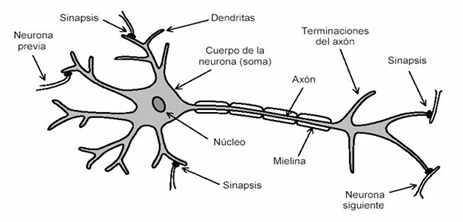
\includegraphics[width=10.5cm]{Sources/neurona.png}
	\captionof{figure}{Neurona biológica}
\end{floatingfigure}

El elemento estructural y funcional más esencial, en el sistema de comunicación neuronal, es la célula nerviosa o neurona. La mayoría de las neuronas utilizas sus productos de secreción como señales químicas (transmisores) para la transmisión de información. Dicha información se envía, entre las distintas neuronas, a través de prolongaciones, formando redes en las cuales se elabora y almacena información.

La misión de las neuronas comprende generalmente cinco funciones parciales:

{\setlength{\baselineskip}{0.7\baselineskip}\begin{itemize}
	\item Las neuronas recogen la información que llega a ellas en forma de impulsos procedentes de otras neuronas o de receptores.
	\item La integran en un código de activación propio de la célula.
	\item La transmiten codificada en forma de frecuencia de impulsos a través de su axón. 
	\item A través de sus ramificaciones el axón efectúa la distribución espacia de los mensajes.
\end{itemize}}

Una Red de Neuronas Artificiales (en adelante, RNA) es un paradigma de procesamiento de información inicialmente inspirado en el modo en el que lo hace el cerebro. El elemento clave de este paradigma es su estructura. Las RNA están compuestas por un cierto número de elementos de procesamiento o neuronas que trabajan al unísono para resolver un problema específico. 

\begin{wrapfigure}{l}{6.1cm}
	\vspace{0.2cm}
		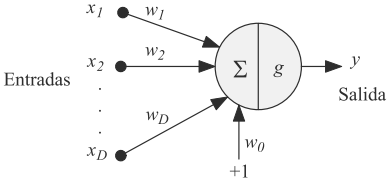
\includegraphics[width=6cm]{Sources/modelo_neurona.png}
		\captionsetup[figure]{margin=0.3cm, justification=centering}
		\captionof{figure}{Modelo matemático de una neurona}\label{modeloneurona}
\end{wrapfigure}

Las redes neuronales actuales se basan en el modelo matemático de neurona propuesto por \textit{McCulloch} y \textit{Pitts} en 1943. En dicho modelo (véase Figura \ref{modeloneurona} ) cada neurona recibe un conjunto de entradas ${x1, x2,...,xD}$ y devuelve una única salida . Además, dentro de una RNA existen numerosas conexiones entre las distintas neuronas que la forman. Estas conexiones simulan las conexiones neuronales del cerebro y, al igual que éstas, pueden establecerse con mayor o menor intensidad. En el caso de las RNA esta intensidad la determinan los pesos sinápticos (o simplemente pesos). De este modo, cada entrada $x_i$ de una neurona se encuentra afectada por un peso $w_i$.

El primer paso para obtener la salida de la neurona es calcular la suma ponderada $a$ de las entradas, llamada activación de la neurona:
$$a = \displaystyle \sum_{i=1}^{D} w_ix_i + w_0$$
Donde w0 es un umbral o sesgo que se utiliza para compensar la diferencia entre el valor medio de las entradas, sobre todo el conjunto de entrenamiento, y el correspondiente valor medio de las salidas deseadas. Posteriormente, a partir de este valor a se obtiene la salida y de la neurona mediante la aplicación de una función, llamada función de activación o de transferencia g(a), es decir:
$$y = g(a) = g\left( \sum_{i=1}^{D}w_ix_i+w_0\right) = g\left( \sum_{i=0}^{D}w_ix_i \right) $$
Donde, como se observa, es posible tratar el umbral $w_0$ como un peso más si se supone una entrada añadida $x_0$ con un valor fijo de 1. Finalmente, también es posible reescribir esta ecuación en notación vectorial como $g(a) = g(w^T x)$, si tomamos $w$ como el vector de pesos y $x$ como el vector de entradas a la red. La función de transferencia empleada en este modelo básico de \textit{McCulloch-Pitts} es la función escalón definida por la ecuación: 
$$\displaystyle g(a) = \left\{ { 0 \mbox{ cuando } x < 0  \atop 1 \mbox{ cuando } a > 0 } \right.$$

En los modelos actuales se escogen otro tipo de funciones, normalmente monótonas y derivables. A continuación se presentarán algunas de ellas.

{\setlength{\baselineskip}{0.7\baselineskip}\begin{itemize}
	\item lineal $g(a)=a$
	\item sigmoidal $g(a) = \displaystyle \frac{1}{1 +e^{-a}}$
	\item tangente hiperbólica $g(a)= \displaystyle \frac{e^a -e^{-a}}{e^a + e^{-a}}$
	\item gaussiana $g(a) = e\left( \displaystyle -\frac{(a-\mu)^2}{2\sigma^2} \right) $
\end{itemize}}

\begin{figure}[H]
	\centering
	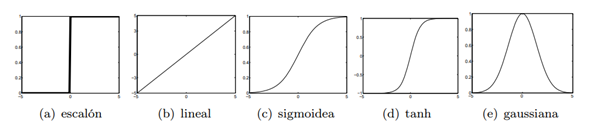
\includegraphics[width=0.8\linewidth]{Sources/funciones_activacion.png}
	\caption{Funciones de activación}
\end{figure}

\subsubsection{Algoritmos genéticos}
Los Algoritmos Genéticos (AG) fueron introducidos inicialmente por Holland en 1975 para abstraer y explicar rigurosamente los procesos adaptativos de los sistemas naturales, así como para el diseño de sistemas artificiales de software que retengan los mecanismos importantes de los sistemas naturales. Fue unos años más tarde cuando su alumno, D. Goldberg, implementó el primer AG aplicado en problemas industriales. Estas y otras aplicaciones creadas por estudiantes de Holland convirtieron los AGs en un campo suficientemente aceptado.

En un AG, las soluciones potenciales al problema se representan normalmente mediante cadenas binarias de bits (0’s y 1’s) de una longitud determinada \emph{long} que vendrá impuesta por el número de variables existentes en la solución y por el número de bits necesarios para codificarlas. Otros términos usados a menudo para denominar una solución del problema en un AG son string o estructura, y, siguiendo el vocabulario de los sistemas biológicos, cromosoma.

Así, los cromosomas están compuestos por unidades binarias que se denominan genes. Al valor de un gen determinado se le denomina alelo, y a su posición en el cromosoma locus. Al paquete genético total se le denomina genotipo, y a la interacción del genotipo con su entorno se le denomina fenotipo, que se traduce en la decodificación del cromosoma para la obtención de una solución alternativa (conjunto de parámetros particulares, o un punto en el espacio de búsqueda). De esta forma, podemos representar un cromosoma $c_i^t$ en una generación (iteración) determinada $t$ como:
{\large $$ c_i^t = \displaystyle (b_{i_1}^t \ldots b_{i_long}^t)$$}
Con $b_{i_j}^t$ $\in$ \{0, 1\}, $j$ = 1,$\ldots$, $long$. El término individuo es frecuentemente utilizado para referirse al conjunto de información genotipo-fenotipo adecuación. Así, podemos representar un individuo $X_i^t$ en una generación $t$, como la terna:
{\large $$ X_i^t = \displaystyle (c_i^t, x_i^t, f_i^t)$$}
Donde $X_i^t$ es la decodificación (fenotipo) del cromosoma $c_i^t$, y $f_i^t$ es la adecuación de la solución al entorno o \textit{fitness}.

\subsubsection{Sistemas expertos}

En la década de los setenta se inicia la explosión de aplicaciones de la IA en términos de sistemas basados en reglas a los que se les llama primero “Sistemas Expertos” y después “Sistemas Basados en Conocimiento”. El reconocimiento de la insuficiencia de la lógica como herramienta única de representación da lugar al desarrollo de otras formas de representación e inferencia mediante redes causales y asociativas (semánticas, neuronales y bayesianas) y marcos, objetos y agentes.

El área de sistemas expertos es una aproximación muy exitosa a la solución de problemas clásicos de AI en la programación de inteligencia. El profesor Edward Feigenbaum de la Universidad de Stanford, pionero en la tecnología de los sistemas expertos, los ha definido como “un programa de computación inteligente que usa el conocimiento y procedimientos de inferencia para resolver problemas que son lo suficientemente difícil como para requerir significativa experiencia humana para su solución, es decir, un sistema experto es un sistema de cómputo que emula la habilidad de tomar decisiones de un especialista humano.

El conocimiento de un sistema experto puede representarse de varias maneras (puede estar encapsulado en reglas y objetos). Un método común de representar el conocimiento es en forma de reglas tipo SI…ENTONCES, como:
\begin{center}
	\textit{SI la luz es roja ENTONCES deténgase.}
\end{center}
Aunque se trata de un ejemplo muy simple, se han construido muchos sistemas expertos significativos expresando en reglas el conocimiento de especialistas.

Los sistemas expertos se han aplicado casi a todos los campos del conocimiento, debido a eso a continuación se mencionarán algunos:


\begin{longtable}[c]{lll} \toprule
	Nombre del S.E.& Área & Descripción\\\midrule
	SPEX & Química & Planear experimentos de biología molecular. \\
	PUFF & Medicina & Diagnosticar enfermedades de los pulmones. \\
	LITHO & Geología & Interpretar los datos de registro de pozos petroleros.\\
	TIMM & Informática & Diagnosticar computadoras DEC.\\\bottomrule
	\caption{Ejemplos de Sistemas Expertos}
\end{longtable}


\subsection{Lógica difusa}\label{seccion:logicadifusa}
Hace más de 50 años, en 1965 Lotfi A. Zadeh, en aquel entonces director del Departamento de Ingeniería Eléctrica de la
Universidad de California en Berkeley, publicó \emph{Fuzzy Sets}. Este artículo describe las matemáticas de los
conjuntos difusos y por extensión de la lógica difusa, y este trabajo le dio nombre a su campo. Zadeh
aplicó la lógica de Lukasiewicz a cada objeto en un conjunto y creó un álgebra completa para conjuntos
difusos. Esta teoría propone \emph{funciones de pertenencia} (o los valores falso y verdadero) sobre el rango
[0.0, 1.0]. 

El ser humano muestra dificultad para tomar decisiones cuando
se tiene información imprecisa. La lógica difusa fue creada para emular la lógica humana y tomar decisiones
acertadas a pesar de la información. Es una herramienta flexible que se basa en reglas lingüísticas
dictadas por expertos. Por ejemplo, la velocidad de un automóvil es una variable que puede tomar distintos
valores lingüísticos, como “alta”, “media” o “baja”. Estas variables lingüísticas están regidas por
reglas que dictan la salida del sistema.
En otras palabras, la lógica difusa es un conjunto de principios matemáticos basados en \emph{grados de
membresía o pertenencia}, cuya función es modelar información. Este modelado se hace con base en
reglas lingüísticas que aproximan una función mediante la relación de entradas y salidas del sistema
(composición). Esta lógica presenta rangos de membresía dentro de un intervalo entre 0 y 1, a diferencia
de la lógica convencional, en la que el rango se limita a dos valores: el cero o el uno.




\subsection{Conjuntos difusos}

El concepto de conjunto difuso fue propuesto por Zadeh(1965): ``Un conjunto difuso es una colección de objetos con un \textit{grado de membresía} continuo. Un conjunto tal, es caracterizado por una \textit{función de membresía} que asigna a cada objeto un grado de membresía en un rango de 0 a 1.'' (p.338).

En teoría clásica de conjuntos, un conjunto tiene unos límites \textit{nítidos} bien definidos (límites \textit{crisp}). Por ejemplo, el conjunto A de los números más grandes que 8 se representa como:

\begin{displaymath}
	A = \lbrace  x \ | \ x > 8 \rbrace
\end{displaymath}

Sin embargo, los conceptos manejados por el ser humano como \textit{frío} y \textit{caliente}, tienen una transición gradual. Así, un conjunto difuso, lidia con la vaguedad inherente de estos conceptos, conteniendo los elementos sólo con un cierto grado de pertenencia.
 
En teoría de conjuntos difusos, los conceptos se asocian a conjuntos difusos (asociando sus \emph{valores de pertenencia}) en un proceso llamado \emph{fuzzificación}. Una vez que tenemos los valores \emph{fuzzificados} podemos trabajar con \emph{reglas lingüísticas} y obtener una salida, que podrá seguir siendo difusa o \emph{defuzzificada} para obtener un valor discreto.

Sea $X$ el \emph{Universo del discurso}, y sus elementos se denotan como $x$; En la teoría clásica de conjuntos se define un conjunto $C$ sobre $X$ mediante la \emph{función característica} de $C$ como $f_c$ .

$$\displaystyle f_c(x) = \left\{ { 1 \mbox{ cuando } x \in C  \atop 0 \mbox{ cuando } x \notin C } \right.$$

Este conjunto mapea el universo $X$ en un conjunto de dos elementos,
donde la función $fc (x)$ es $1$ si el elemento $x$ pertenece al conjunto
$C$ y $0$ si el elemento $x$ no pertenece al conjunto $C$.

Si generalizamos esta función para que los valores asignados a los
elementos del conjunto caigan en un rango particular y así indicar
el grado de pertenencia de los elementos a ese conjunto, tendremos
una \textbf{función de pertenencia} de un determinado conjunto difuso.
La función de pertenencia $\mu_A $ por la que se define un conjunto difuso $A$,
Sería:

\begin{displaymath}
\mu_A = X \rightarrow \left[ 0,1 \right]
\end{displaymath}


Donde $\mu_A(x) = 1$ si $x$ está totalmente en $A$,
$\mu_A(x) = 0$ si $x$ no está en $A$
y $ 0 < \mu_A(x) < 1 $ si $x$ está parcialmente en $A$.
Este valor entre 0 y 1 representa el grado de pertenencia $\mu$ al conjunto $A$.


\textit{Definición formal}\\
Un conjunto difuso $A$ definido en el universo de discurso $U$ es caracterizado por una función de membresía $\mu_A : U \rightarrow [0,1]$ que asocia a cada elemento $u$ de $U$ un valor $\mu_A(u)$ en el intervalo [0,1], con $\mu_A(u)$ representando el grado de membresía de $u$ en $A$.

Algunas características:
{\setlength{\baselineskip}{0.7\baselineskip}\begin{description}
	\item El soporte de A son los puntos en $U$ en los cuales $\mu_A(u)$ es positivo.
	\item La altura de A es el valor máximo de $\mu_A(u)$ sobre $U$.
	\item El punto de cruce de A es un punto en $U$ donde el valor de membresía en $A$ es $0.5$
\end{description}}





\subsubsection{Principio isomorfo}

Es bien conocido que la teoría de conjuntos, el \textit{Álgebra booleana} y la Lógica tradicional son isomorfas, bajo transformaciones adecuadas. Esto significa que tienen una estructura subyacente similar, y que por tanto, las definiciones que se hagan en una de las tres teorías se pueden llevar a las otras dos, mediante las transformaciones adecuadas.
En el siguiente cuadro se muestra la correspondencia de algunos operadores.\\\\


\begin{longtable}{|c|c|c|} 
	\hline
	Teoría de conjuntos & Álgebra booleana & Lógica tradicional \\ \hline
	Intersección & Conjunción & AND \\ \hline
	Unión & Disyunción & OR \\ \hline
	Complemento & Negación & NOT \\ \hline
	\caption{Correspondencia entre operadores} \label{table:tblop}
\end{longtable}

Ahora bien, el razonamiento lógico consiste en la combinación de proposiciones para producir nuevas proposiciones; así, la combinación de las proposiciones \textit{X es A} y  \textit{Y es B} mediante el operador \textit{AND} da como resultado la proposición \textit{X es A AND Y es B}. El cuadro \ref{table:tblop} sugiere que puede representarse esta combinación mediante un operador análogo a la intersección de conjuntos.

Lo anterior es posible porque en lógica tradicional toda proposición puede tener uno de dos valores, \textit{verdadero} o \textit{falso}, lo que corresponde en la teoría de conjuntos discretos a los únicos dos valores que puede tomar la función de pertenencia para cualquier conjunto: 1 ó 0.


Ahora bien, en lógica difusa una proposición puede representarse por un conjunto difuso \textit{X es A} corresponde a un conjunto A con función de pertenencia $\mu_A(x)$, mientras \textit{Y es B} corresponde a un conjunto B con función de pertenencia $\mu_B(x)$, y la combinación de estas dos proposiciones con el operador \textit{AND}, es decir, la proposición \textit{X es A AND Y es B} corresponde a un nuevo conjunto difuso \textit{A AND B} con función de pertenencia:

\begin{displaymath}
\mu_{A \cap B}(x,y) =  \min(\mu_A(x),\mu_B(y))
\end{displaymath}

En donde se ha utilizado el operador $\min$ parara efectuar la intersección de los dos conjuntos, pero en general podría haberse utilizado cualquier norma T.

Nótese que los universos de discurso sobre los cuales están definidos los conjuntos A y B no son necesariamente el mismo; son, por ejemplo U y V respectivamente, mientras el conjunto $A \cap B$ está definido sobre el universo $U \times V$.

En forma análoga, al operador lógico $OR$ puede hacerse corresponder a una \textit{norma S}, mientras al operador lógico $NOT$ puede hacerse corresponder el complemento.









\subsection{Operaciones de conjuntos difusos}

Las tres operaciones básicas entre conjuntos discretos: \emph{unión, intersección y complemento}, se definen también para los conjuntos difusos, intentando mantener el significado de tales operaciones. La definición de estas operaciones se hace empleando el concepto de función de pertenencia de los conjuntos.

\subsubsection{Intersección}

Dado dos conjuntos difusos $A$ y $B$ con funciones de pertenencia $\mu_A(x)$ y $\mu_B(x)$, respectivamente.
La intersección $A \cap B$ puede representarse en general como una función
$T:[0,1] \times [0,1] \rightarrow [0,1]$ o como un operador binario $\vartriangle$, tal que:

%La intersección es un nuevo conjunto difuso $A \cap B$ con una función de pertenencia:

\begin{displaymath}
\mu_{A \cap B}(x,y) = T [ \mu_A(x), \mu_B(y) ] = \mu_A(x) \vartriangle \mu_B(y)
\end{displaymath}

Donde $T$, debe satisfacer las siguientes propiedades:

\begin{enumerate}
	\item \textsl{Elemento unidad:} $T(a,1) = a$ y $T(a,1)=T(1,a)=a$
	\item \textsl{Conmutatividad:} $T(a,b) = T(b,a)$
	\item \textsl{Monotonicidad:} Si $a \leq c$ y $b \leq d$ entonces $T(a,b) = T(c,d)$
	\item \textsl{Asociatividad:} $T(T(a,b),c) = T(a,T(b,c))$
\end{enumerate}

Todo operador que satisfaga las propiedades anteriores se conoce como una \textbf{Norma Triangular} o \textbf{Norma T} y representa la intersección de dos conjuntos difusos. Algunas \textit{normas T} ampliamente utilizadas son:

\begin{itemize}
	\item \textsl{Mínimo:} $T_{min}(a,b) = min(a,b)$
	\item \textsl{Producto algebraico:} $T_{ap}(a,b) = ab$
	\item \textsl{Diferencia limitada (o de Lukasiewick)}: $T_{bp}(a,b) = max(0, a+b-1)$
\end{itemize}





\subsubsection{Unión}
Dado dos conjuntos difusos $A$ y $B$ con funciones de pertenencia $\mu_A(x)$ y $\mu_B(x)$, respectivamente.
La unión $A \cup B$ puede representarse en general como una función
$S:[0,1] + [0,1] \rightarrow [0,1]$ o como un operador binario $\bot$, tal que:

%Dado nuevamente, dos conjuntos difusos $A$ y $B$, con funciones de pertenencia $\mu_A(x)$ y $\mu_B(x)$, respectivamente. La unión se define como un nuevo conjunto difuso $A \cup B$ con una función de pertenencia:

\begin{displaymath}
\mu_{A \cup B}(x,y) = S \left[ \mu_A(x), \mu_B(y) \right] = \mu_A(x) \ \bot \ \mu_B(y)
\end{displaymath} 

Donde $S$, debe satisfacer las siguientes propiedades:

\begin{enumerate}
	\item \textsl{Elemento Neutro:} $S(1,1)=1$ y $S(a,0) = S(0,a) = a$
	\item \textsl{Conmutatividad:} $S(a,b) = S(b,a)$
	\item \textsl{Monotonicidad:} Si $a \leq c$ y $b \leq d$ entonces $S(a,b) = S(c,d)$
	\item \textsl{Asociatividad:} $S(S(a,b),c) = S(a,S(b,c))$
\end{enumerate}


Todo operador que satisfaga las propiedades anteriores se conoce como una \textbf{Conorma T} o \textbf{Norma S} y representa la unión de dos conjuntos difusos. Algunas \textit{normas S} ampliamente utilizadas son:

\begin{itemize}
	\item \textsl{Máximo:} $S_{max}(a,b) = max(a,b)$
	\item \textsl{Producto:} $S_{as}(a,b) = (a+b) - (a \times b)$
	\item \textsl{Suma limitada (o de Lukasiewick)}: $S_{bs}(a,b) = min(a+b,1)$
\end{itemize}

\subsubsection{Complemento}
Dado un conjunto $A$, con función de pertenencia $\mu_A(x)$.
El complemento $\neg A$ puede generalizarse considerándolo como una función
$N:[0,1] \rightarrow [0,1]$, tal que:


\begin{displaymath}
	\mu_{\neg A}(x) = N( \mu_A(x) )
\end{displaymath}

La operación de complemento, a la que llamaremos \textbf{Norma N}, también debe cumplir ciertas propiedades:

\begin{enumerate}
	\item \textsl{Condición limite o frontera:} $N(0) = 1$ y $N(1) = 0$.
	\item \textsl{Monotonicidad:} si $a \leq b$ entonces $N(a) \geq N(b)$.
	\item \textsl{Continuidad:} la función de complemento $N(a)$ es continua.
	\item \textsl{Involutividad:} $N(N(a)) = a $
\end{enumerate}

Al igual que con la unión y la intersección, también para el complemento, existen gran variedad de clases.
Algunas \textit{normas N} más utilizadas son:

\begin{enumerate}
	\item \textsl{Clásico:} $N_{c}(a) = 1 - a$
	\item \textsl{Sugeno:} $N_{s}(a) = \frac{1-a}{1+sa}$ con $s \in (-1,\infty)$
	\item \textsl{Yager:} $N_{w}(a) = (1-a^w)^{1/w}$ con $w \in (0, \infty)$
\end{enumerate}



\subsection{Funciones de membresía}\label{cap:membershipfunction}

Para definir un conjunto difuso $A$, hay que definir su \textit{función de membresía} o \textit{función de pertenencia}.
Supongamos una función de pertenencia: $\mu_A(x)$, la imagen de la función es la curva que define el grado de pertenencia de cada elemento $x$ al conjunto $A$.

Para la correcta representación de los grados de pertenencia de cada uno de los elementos que conforman el conjunto difuso, lo más natural es extraer los datos de los fenómenos que se va a representar y con ellos, elegir y ajustar una función de membresía adecuada. De otra manera existen metodologías que permiten asignar grados de membresía a cada uno de los elementos del conjunto.

Algunas de las funciones de membresía básicas son las siguientes.

\paragraph{Triangular.}
\begin{wrapfigure}{r}{0pt}
	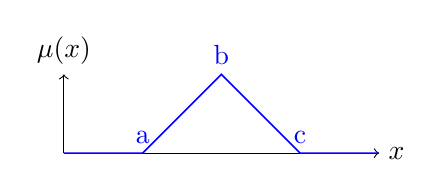
\begin{tikzpicture}
		\draw[->] (0,0) -- (4,0) 	node[right] {$x$} 		coordinate (x axis);
		\draw[->] (0,0) -- (0,1) 	node[above]	{$\mu(x)$} 	coordinate (y axis);
		\draw[blue,semithick] (0,0) -- (1,0) node[above] {a} -- (2,1) node[above] {b} -- (3,0) node[above] {c} -- (4,0);
	\end{tikzpicture}
	\captionsetup{margin=1cm,justification=centering}	
	\caption{Función triangular}
	\label{fig:trimf}
\end{wrapfigure}
La imagen de la función, como su nombre lo indica, asemeja un triángulo. Realmente la función está compuesta por dos líneas rectas, una con pendiente positiva hasta alcanzar la unidad, y otra con pendiente negativa, hasta llegar a 0. Está definida por tres parámetros \textit{a, b, c} donde $ a \leq b \leq c$. Estos parámetros definen los vértices de la función.\\\\
Su definición matemática es la siguiente:
$$  f(x;a,b,c)= \left\lbrace \begin{array}{lcl}
0	& \mbox{si} & x  \leq a \\ [.30cm]
{\displaystyle \frac{x-a}{b-a}} & \mbox{si} & a \leq x \leq b \\ [.45cm]
%{\scriptstyle (x-a)/(b-a)} & \mbox{si} & a \leq x \leq b \\ [.15cm]
{\displaystyle \frac{c-x}{c-b}} & \mbox{si} & b \leq x \leq c \\ [.45cm]
%{\scriptstyle (c-x)/(c-b)} & \mbox{si} & b \leq x \leq c \\ [.15cm]
0 & \mbox{si} & x \geq c \\
\end{array}				
\right.
$$

La función triangular es adecuada para definir situaciones en las que se tiene un valor óptimo central, el cual se va perdiendo conforme se aleja de él. Un ejemplo de esta situación es la temperatura corporal, esta tiene un valor óptimo de $36\,^{\circ}\mathrm{C}$, pero por debajo de $35\,^{\circ}\mathrm{C}$ o por encima de $37\,^{\circ}\mathrm{C}$ se podría considerar peligrosa.


\paragraph{Trapezoidal.}
\begin{wrapfigure}{r}{0pt}
	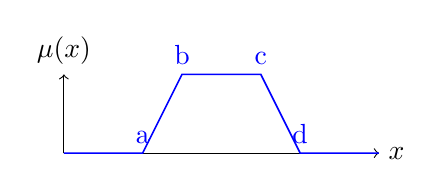
\begin{tikzpicture}
		\draw[->] (0,0) -- (4,0) 	node[right] {$x$} 		coordinate (x axis);
		\draw[->] (0,0) -- (0,1) 	node[above]	{$\mu(x)$} 	coordinate (y axis);		
		\draw[blue,semithick] (0,0) -- 	(1  ,0)	node[above] {a} --
		(1.5,1) node[above] {b} --
		(2.5,1)	node[above] {c} --
		(3,0)	node[above] {d} --
		(4,0);
	\end{tikzpicture}
	\captionsetup{margin=1cm,justification=centering}	
	\caption{Función triangular}
	\label{fig:trapmf}
\end{wrapfigure}

Una generalización de la función triangular es la función trapezoidal, que a diferencia de la triangular, tiene un núcleo más amplio. Esto es, el intervalo donde el valor de membresía es igual a 1 se extiende entre los vértices
$b$ y $c$.
La función está definida por cuatro parámetros \textit{a, b, c, d} donde $ a \leq b \leq c \leq  d$. En la figura \ref{fig:trapmf} se aprecia el trapecio que forman estos cuatro vértices.\\\\
Su definición matemática es la siguiente:

$$  f(x;a,b,c,d)= \left\lbrace \begin{array}{lcl}
						0		& \mbox{si} & x  \leq a \\ [.30cm]
{\displaystyle \frac{x-a}{b-a}} & \mbox{si} & a \leq x \leq b \\ [.45cm]
						1		& \mbox{si} & b \leq x \leq c \\ [.30cm]
{\displaystyle \frac{c-x}{c-b}} & \mbox{si} & c \leq x \leq d \\ [.45cm]
						0 		& \mbox{si} & x \geq d \\
\end{array}
\right.
$$

La forma de esta función es utilizada cuando hay un rango de valores óptimos. Un ejemplo de esto es la temperatura ambiente. Hay un rango de temperaturas que podemos considerar adecuadas, pero por debajo de este rango las personas comienzan a sentir frío, y por encima de él se consideraría un ambiente caluroso.


\paragraph{Gaussiana.}
\begin{wrapfigure}{r}{0pt}
	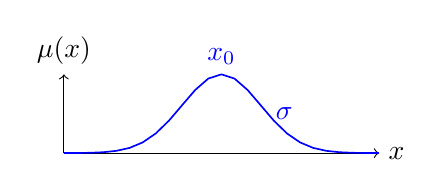
\begin{tikzpicture}[domain=0:8, xscale=0.5]
	\draw[->] (0,0) -- (8,0) 	node[right] {$x$} 		coordinate (x axis);
	\draw[->] (0,0) -- (0,1) 	node[above]	{$\mu(x)$} 	coordinate (y axis);
	
	\draw[blue, semithick]	plot(\x,{  exp( -1/2 * pow( ( (\x - 4) / 1 ) ,2) ) });
	\draw[blue] (4,1) node[above] {$x_0$};
	\draw[blue] (5.6,0.3) node[above] {$\sigma$};
	
	\end{tikzpicture}
	\captionsetup{margin=1cm,justification=centering}	
	\caption{Función gaussiana}
	\label{fig:gaussmf}
\end{wrapfigure}

La \textit{función gaussiana} es una función simétrica que juega el papel de la función triangular, solo que esta pertenece al grupo de las funciones con derivada continua. Si observamos la figura \ref{fig:gaussmf} podemos ver como la gráfica asemeja un triángulo suavizado, es decir, los vértices no tienen cambios abruptos sino graduales.\\\\
Su definición matemática es la siguiente:
\begin{displaymath}
f(x;a,x_0)=  e^{\displaystyle -\frac{1}{2} \left(  \frac{x-x_0}{a} \right)^2 }
\end{displaymath}
Donde
{\setlength{\baselineskip}{0.7\baselineskip}\begin{description}
	\item $x_0$ determina el centro o punto de cruce y,
	\item $a$ determina el ancho o la pendiente.
\end{description}}

%test campana generalizada
\paragraph{Campana generalizada.}

\begin{wrapfigure}{r}{0pt}
		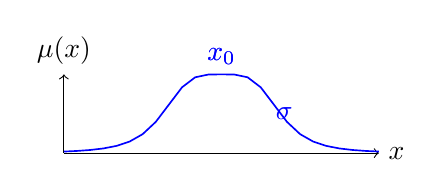
\begin{tikzpicture}[domain=0:8, xscale=0.5]
			\draw[->] (0,0) -- (8,0) 	node[right] {$x$} 		coordinate (x axis);
			\draw[->] (0,0) -- (0,1) 	node[above]	{$\mu(x)$} 	coordinate (y axis);
			
			\draw[blue, semithick]	plot(\x,{ 1 / ( 1 + pow( (\x - 4)/ 1.5 , 2 * 2) ) });
			\draw[blue] (4,1) node[above] {$x_0$};
			\draw[blue] (4,1) node[above] {$x_0$};
			\draw[blue] (5.6,0.3) node[above] {$\sigma$};
		\end{tikzpicture}
		\captionsetup{margin=1cm,justification=centering}	
		\caption{Función Campana generalizada}
		\label{fig:gbellmf}
\end{wrapfigure}
Esta función al igual que la anterior, es una función simétrica con derivada continua. Juega el papel de una función trapezoidal, si observamos la figura \ref{fig:gbellmf}, podemos ver como la gráfica asemeja un trapecio suavizado, es decir, los vértices no tienen cambios abruptos sino graduales.\\\\
Su definición matemática es la siguiente:

\begin{displaymath}
f(x;a,b,x_0)= \frac{1}{1 + \left(  \frac{x-x_0}{a}  \right)^{2b}}
\end{displaymath}
Donde
{\setlength{\baselineskip}{0.7\baselineskip}\begin{description}
	\item $x_0$ determina el centro o punto de cruce,
	\item $a$ determina el ancho y,
	\item $b$ determina la pendiente.
\end{description}}


\paragraph{Sigmoidal.}

\begin{wrapfigure}{r}{0pt}
	\begin{tikzpicture}[domain=0:8, xscale=0.5, yscale=1]
		\draw[->] (0,0) -- (8,0) 	node[right] {$x$} 		coordinate (x axis);
		\draw[->] (0,0) -- (0,1) 	node[above]	{$\mu(x)$} 	coordinate (y axis);
		\draw[blue]	plot(\x,{ 1 / ( 1 + exp( -1 * -2 * (\x-3.5)  ) ) });
	\end{tikzpicture}
	\captionsetup{margin=1cm,justification=centering}	
	\caption{Función Sigmoidal}
	\label{fig:sigmf}
\end{wrapfigure}

Una sigmoidal es una función con derivada continua y abierta. Su gráfica recuerda la forma de un escalón. Tiene un parámetro $a$ que determina su pendiente, es decir, determina la suavidad de la transición entre los valores de membresía 0 a 1. Además el parámetro a también determina si la función abrirá por la izquierda o por la derecha. Un valor positivo de $a$ genera un gráfica abierta por la derecha
y un valor negativo genera que l gráfica se abra por la izquierda.
En la imagen \ref{fig:sigmf} podemos observar una función sigmoidal abierta por la izquierda.\\\\
Su definición matemática es la siguiente:
\begin{displaymath}
	f(x;a,x_0) = \frac{1}{1+e^{-a(x-x_0)}}
\end{displaymath}
Donde
{\setlength{\baselineskip}{0.7\baselineskip}\begin{description}
	\item $x_0$ determina el centro o punto de cruce y,
	\item $a$ determina la pendiente.
\end{description}}

\subsection{Variables lingüísticas}
Una variable lingüística adopta términos lingüísticos que permiten describir el estado de un objeto o fenómeno usando un lenguaje natural(o artificial); estos términos se pueden representar mediante conjuntos difusos. Una variable numérica toma valores numéricos, por ejemplo: \textit{carros = 2}, mientras que una variable lingüística toma valores lingüísticos: carros es \textit{``pocos''}.

De manera más formal: Los valores de una variable lingüística $X$ son las etiquetas $T(x)$ de los subconjuntos difusos en U(conjunto universo). Las etiquetas pueden tener la forma de frases o sentencias en lenguaje natural o artificial. Por ejemplo, si U es la colección de enteros correspondiente a las edades de un grupo de personas:
$$U = 10 + 1 + 2 + ... + 70$$
y la edad es una variable lingüística llamada \textit{x} definida en \textit{U}, entonces los valores de \textit{x} podrían ser \textit{niño, joven, adulto joven, adulto, anciano}, etc. Donde los posibles valores son las etiquetas de los conjuntos difusos que caracterizan las edades (véase la fig. \ref{fig:variableling}).

\begin{figure}[!h]
	\centering
	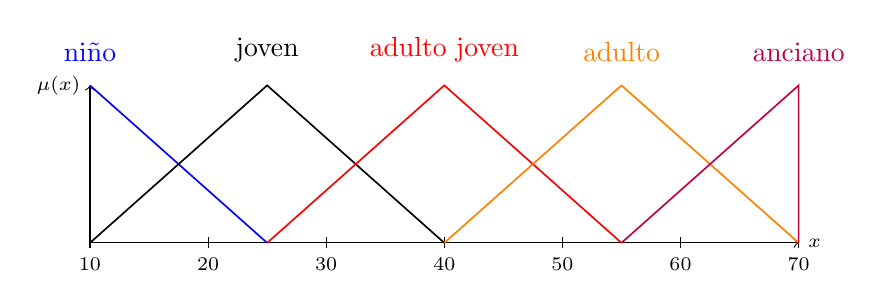
\begin{tikzpicture}[yscale=2, xscale=1.5]
		\draw[->] (1,0) -- (7,0) 	node[right] {${\scriptstyle x}$} 		coordinate (x axis);
		\draw[->] (1,0) -- (1,1) 	node[left]	{${\scriptstyle \mu(x)}$} 	coordinate (y axis);
		
		\foreach \x in {1, 2, ..., 7}
			\draw[xshift=\x cm] (0pt,1pt) -- (0pt,-1pt) node[below] {{\scriptsize \x0}};
		
		
		\draw[blue, semithick] (1,1) node[above=5pt] {niño} -- (2.5,0);
		\draw[black, semithick]	(1,0) -- (2.5,1) node[above=5pt] {joven} -- (4,0);
		\draw[red,semithick] (2.5,0) -- (4,1) node[above=5pt] {adulto joven}  -- (5.5,0);
		\draw[orange,semithick] (4,0) -- (5.5,1) node [above=5pt] {adulto} -- (7,0);
		\draw[purple,semithick] (5.5,0) -- (7,1) node [above=5pt] {anciano} -- (7,0);
	\end{tikzpicture}
	\caption{Variable lingüística \emph{edad} llamada $x$}
	\label{fig:variableling}
\end{figure}

El significado de un término lingüístico $T(x)$ es caracterizado mediante una \textit{función de compatibilidad o membresía}: $C : U \rightarrow [0,1]$, la cual, asocia la compatibilidad (o grado de pertenencia) de cada $u$ en $U$, con $T(x)$. Así, la compatibilidad de una edad de \textit{27 años} con el término lingüístico \textit{joven} podría ser 0.7, mientras que una edad de \textit{35 años} podría ser de 0.2.

El concepto de variable lingüística proporciona un medio para definir de manera aproximada los fenómenos que son demasiado complejos o muy imprecisos como para ser receptivos de una descripción convencional en términos cuantitativos.

Una variable lingüística está caracterizada mediante la quíntupla:
$$(X,T(x),U,G,M)$$
Donde
{\setlength{\baselineskip}{0.7\baselineskip}\begin{description}
	\item $X$ es el nombre de la variable.
	\item $T(X)$ es el conjunto de términos o valores lingüísticos.
	\item $U$ es el universo de discurso.
	\item $G$ es la regla sintáctica que genera los términos en $T(x)$; y,
	\item $M$ es una regla semántica que socia cada valor lingüístico $X$ con su correspondiente significado $M(X)$, siendo $M(X)$ un conjunto difuso en $X$.
\end{description}}

Hay varios aspectos básicos que es necesario tomar en cuenta al momento de definir de una variable lingüística.

Primero, Es importante entender que la noción de membresía es distinta a la de probabilidad. Así, la declaración de que la membresía de la edad de \emph{28 años} al conjunto difuso \emph{joven} es de 0.7, no tiene relación con la probabilidad de que la edad sea o no 28.
La interpretación correcta es que el valor de membresía 0.7, es simplemente una indicación subjetiva de \emph{qué tanto encaja} la edad de ``28 años'' (\textit{en una escala de 0 a 1}) con el concepto ``joven''.
%La interpretación correcta del valor de membresía 0.7, es que, simplemente es una indicación subjetiva de \emph{en qué grado} (\textit{en una escala de 0 a 1}) la edad de ``28 años'' encaja en el concepto ``joven''.

Segundo, normalmente asumiremos que una variable lingüística está \emph{estructurada} tomando en cuenta dos reglas:
\begin{description}
	\item[Regla (i).] La regla sintáctica, esta especifica la manera en que se generan los términos lingüísticos de la variable.
	En relación a esta regla, normalmente asumiremos que los términos de la variable son generados por una gramática de contexto libre.
	\item[Regla(ii).] La regla semántica, que especifica el proceso para computar el significado de cualquier término lingüístico dado. Aquí, observamos que un valor típico de una variable lingüística involucra lo que llamamos términos primarios (joven y viejo) que son a su vez, subjetivos y dependientes de contexto. Por lo que se asume que el significado de dichos términos es conocido \emph{a priori}.
\end{description}

En resumen, al momento de definir una variable lingüística $(X,T(x),U,G,M)$, se asume que $G$ es una gramática libre de contexto, además que,
cualquier significado $M(x)$  generado por $M$ es subjetivo y conocido \emph{a priori}. Por lo que normalmente $M$ y $G$ se omitirán en la definición.

Tomando en cuenta lo anterior, una variable lingüística se define básicamente por la siguiente tripla.
$$(X,T(x),U)$$
Donde:
{\setlength{\baselineskip}{0.7\baselineskip}\begin{description}
	\item $X$ es el nombre de la variable.
	\item $T(x)$ es el conjunto de términos o valores lingüísticos.
	\item $U$ es el universo de discurso.
\end{description}}


 
\subsection{Sistema difuso}
Un sistema de inferencia difuso (\textit{FIS}) consta, conceptualmente, de tres etapas. En la primer etapa se transforman (fuzzifican) las variables de entrada obteniendo valores de difusos. Posteriormente dichos valores son manejados por un sistema de inferencia que genera una salida, también difusa, a partir de las reglas establecidas y los propios valores de entrada. Finalmente el resultado pasa por un proceso llamado defuzzificación, a través del cual, se obtiene la salida real del sistema ya en valores concretos. La figura \ref{fig:digfis} muestra el diagrama esquemático del controlador
difuso.

\begin{figure}[H]
	\centering
	\begin{tikzpicture}[scale=2]
	
	\node[draw,rectangle] (fl) at (0,0) {Reglas difusas};
	\node[draw,rectangle] (fz) [left= of fl] {Fuzzificador};
	\node[draw,rectangle] (df) [right= of fl] {Defuzzificador};
	\node[draw,rectangle] (fe) [below= of fl] {Motor de inferencia};
	
	\path (fl) edge[<->] (fe);
	\path (fz) edge[->] (fl);
	\path (fl) edge[->] (df);
	\end{tikzpicture}
	
	\caption{Diagrama esquemático de un sistema de inferencia difuso}
	\label{fig:digfis}
\end{figure}



\subsubsection*{Fuzzificación}
La primera etapa se basa en un proceso donde las variables tienen un grado de incertidumbre metalingüístico. Por lo tanto, el rango de valores (\textit{universo de discurso}) de cada variable puede clasificarse por conjuntos difusos\footnote{Para más información véase la sección \ref{cap:membershipfunction} \textit{Funciones de membresía}.}, por ejemplo \textit{baja, media, alta}.
Cuando el sistema obtiene variables, pasan por un proceso de \textit{fuzzificación}
que consiste en pasar dichos valores a un rango de pertenencia entre cero (0) y uno (1).
Se busca determinar el grado de pertenencia del valor de entrada a un conjunto difuso.
Los conjuntos difusos son caracterizados mediante funciones de membresía ajustadas a las necesidades del sistema. La imagen \ref{fig:fuzzify} muestra la interpretación grafica de la fuzzificación.

\begin{figure}[H]
	\centering
	
	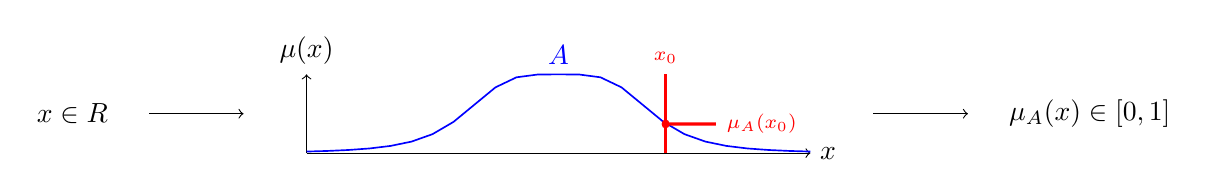
\begin{tikzpicture}[domain=0:8, xscale=0.8]
	
	\draw (-3,0.5) node[left] {$ x \in \mathbb{R} $};
	\draw[->] (-2.5,0.5) -- (-1,0.5);
	
	\draw[->] (9,0.5) -- (10.5,0.5);
	\draw (11,0.5) node[right] {$\mu_A(x) \in [0,1] $};
	
	\draw[->] (0,0) -- (8,0) 	node[right] {$x$} 		coordinate (x axis);
	\draw[->] (0,0) -- (0,1) 	node[above]	{$\mu(x)$} 	coordinate (y axis);
	
	
	\draw[blue, semithick]	plot(\x,{ 1 / ( 1 + pow( (\x - 4)/ 1.5 , 2 * 2) ) });
	
	\draw[red, very thick,font=\scriptsize] (5.7,1) node[above] {$x_0$} -- (5.7,0);
	\draw[red, very thick,font=\scriptsize] (5.7,0.37) circle[radius=1pt, right] -- (6.5,0.37) node[right] {$\mu_A(x_0)$};
	
	
	
	\draw[blue] (4,1) node[above] {$A$};
	
	
	\end{tikzpicture}
	\captionsetup{margin=1cm,justification=centering}	
	\caption{Fuzzificación de un valor concreto}
	\label{fig:fuzzify}
\end{figure}

\subsubsection*{Reglas difusas}
%\subsection{Reglas difusas}
En lógica difusa las proposiciones del tipo ``\ifthen{temperatura}{alta}{ventilador}{máximo}'' son usadas para modelar el conocimiento del experto sobre un fenómeno en un lenguaje natural y cotidiano. A estas proposiciones que operan sobre conjuntos difusos se les conoce como reglas difusas.

El objetivo de las reglas difusas es capturar el conocimiento empírico del experto y al conjunto de reglas se le denomina Base de Conocimientos.

Supongamos una proposición sencilla:
\begin{center}
	\ifthen{x}{a}{y}{b}.
\end{center}

En los sistemas de reglas clásicos, si el antecedente es cierto, el consecuente también lo es. En un sistema difuso donde el antecedente es difuso, todas las reglas se ejecutan parcialmente, el consecuente es cierto, pero solo en cierto grado.

\subsubsection*{Inferencia}
En la segunda etapa se proponen reglas lingüísticas (\textit{inferencia}) que servirán para inferir la salida del sistema.
El grado de pertenencia de cada una de las variables se evalúa en un conjunto de
reglas de inferencia. Dichas reglas de inferencia fueron determinadas con ayuda de un experto. El conjunto
de reglas de inferencia determina una consecuencia, es decir, asigna un grado de pertenencia a un
conjunto difuso que caracteriza a las salidas.

\begin{figure}[H]
	\centering
	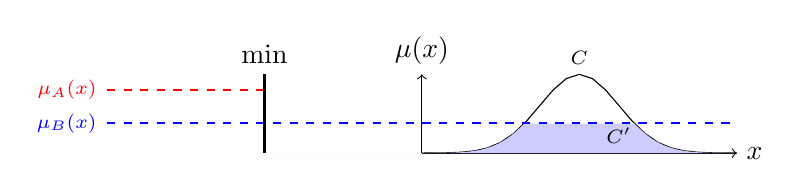
\begin{tikzpicture}[]

	
	\draw[->] (0,0) -- (4,0) 	node[right] {$x$} 		coordinate (x axis);
	\draw[->] (0,0) -- (0,1) 	node[above]	{$\mu(x)$} 	coordinate (y axis);

	\draw plot[blue!30!white,domain=0:4, variable=\x] (\x,{  exp( -1/2 * pow( ( (\x - 2) / 0.5 ) ,2) ) });
		
	\fill [blue!20!white, domain=0:4, variable=\x]
		(-2,0)
		-- plot[domain=0:1.3](\x,{  exp( -1/2 * pow( ( (\x - 2) / 0.5 ) ,2) ) })
		-- plot[domain=2.7:4](\x,{  exp( -1/2 * pow( ( (\x - 2) / 0.5 ) ,2) ) })
		-- (2,0)
		-- cycle;
		
		\draw[red, thick,font=\scriptsize,dashed] (-4,0.8) node[left] {$\mu_A(x)$} -- (-2,0.8);
		\draw[blue, thick,font=\scriptsize,dashed] (-4,0.38) node[left] {$\mu_B(x)$} -- (4,0.38);
		
		\draw[black, very thick] (-2,1) node[above] {min} -- (-2,0);
		
		\draw[font=\scriptsize] (2,1) node[above] {$C$};
		\draw[font=\scriptsize] (2.5,0.45) node[below] {$C'$};
	\end{tikzpicture}
	\captionsetup{margin=1cm,justification=centering}	
	\caption{Inferencia del conjunto resultado C}
	\label{fig:inference}
\end{figure}

En la imagen \ref{fig:fuzzify} se aprecia gráficamente un ejemplo de un proceso de inferenciación, a saber, de tipo mamdani. Existen varios mecanismos de inferencia, la elección de uno de ellos dependerá de la situación. Algunos de los métodos de inferencia más usados son:
{\setlength{\baselineskip}{0.7\baselineskip}\begin{description}
		\item Mamdani.
		\item Sugeno.
		\item Tsukamoto.
\end{description}}
\subsubsection*{Defuzzificación}
Una vez obtenidas las consecuencias, la tercera etapa es un proceso para determinar los valores
óptimos de salida, conocido como defuzzificación, y que consiste en pasar el grado de pertenencia,
proveniente de la consecuencia de las regla de inferencia (\textit{conjunto consecuencia}), a un valor nítido o real. Para hacer
eso, previamente se sintonizaron funciones de membresía de cada una de las salidas con el fin de
obtener un valor cuantificable. 



Al final el control entregará valores nítidos o reales, consecuencia de las reglas lingüísticas previamente
estructuradas, con lo cual este sistema interpretará las órdenes y realizará las acciones
pertinentes.





\newpage

\section{Estado del arte}\label{table:estadodelarte}

\begin{center}
	\begin{longtable}{|p{3.0cm}|p{7.4cm}|p{5.0cm}|}
		

		
		\hline Artículo & Descripción & Resultado \\ \hline
		\endfirsthead
		
		\multicolumn{3}{c}{{\tablename\ \thetable{}: Continúa de la página anterior}}\\

		\hline Articulo & Descripción & Resultado \\ \hline
		\endhead
		
		\hline \multicolumn{3}{|r|}{{\tablename\ \thetable{}: Continúa en la siguiente página...}}\\ \hline
		\endfoot
		
		\hline \multicolumn{3}{|r|}{{ \tablename\ \thetable{}: Estado del arte }}\\ \hline

		\endlastfoot
		

		
		Un enfoque de semáforo inteligente utilizando algoritmos de visión computacional en una intersección aislada para optimizar el flujo vehicular.\cite{garciag} \newline \emph{(08/02/2017)} &
		El sistema consta de una serie de cámaras que son colocadas en una intersección vehicular, mismas que detectan el movimiento de los autos mediante algoritmos de visión computacional.
		Posteriormente, la información recabada por las cámaras es enviada a un sistema de control inteligente, el cual se encarga de analizar y determinar cuándo cambiar la luz del semáforo.&
		Solo se evaluó la detección de cantidad de carros de una imagen y se logró tener el resultado correcto. El siguiente paso es la evaluación de toma de decisiones.\\ \hline
		
		
		Control de tráfico vehicular automatizado utilizando Lógica Difusa.\cite{alvaroer} \newline \emph{(2008)} &
		Se ha utilizado la librería de Matlab Fuzzy. Se analizó una intersección de dos avenidas que cuentan con tres periodos de semáforos.  Todos los diseños del programa de control fueron implementados inicialmente en Matlab utilizando la librería Fuzzy, como referencia. En base a ello se ha realizado la implementación del algoritmo final en un dispositivo de hardware: PIC, para realizar el procesamiento de la información utilizando el lenguaje de programación PIC basic.&
		Presenta muchos altibajos en la eficiencia llegando en el peor de los casos a una eficiencia de menos del 30\%, lo cual es inaceptable.\\ \hline
		
		Semáforos inteligentes para la regulación del tráfico vehicular.\cite{bencesramos} \emph{(07/2014)}&
		La Investigación desarrolla un Sistema de Semáforo Inteligente (SSI), basado en lógica difusa, que según la densidad vehicular capturada por cámaras web, permiten organizar los cambios de luces en función de las condiciones que se presenten en la zona.
		Este trabajo es una aplicación de lógica difusa, y está basado en visión por computador, cámaras web que permiten la entrada de datos, lenguaje de programación Python, para el procesamiento de imágenes algoritmos de visión, como es OpenCV y Highgui, así como del Microcontrolador PIC 18F2550.&
		Mediante el desarrollo de un prototipo se simuló el flujo de vehículos que cruzan por dos intersecciones. El uso del sistema de semáforos inteligentes con lógica difusa ha permitido regular el tráfico vehicular, obteniendo resultados muy favorables, en donde los semáforos permiten dar tiempos variables dependiendo de la densidad vehicular en tiempo real, logrando así mayor fluidez del flujo vehicular.\\ \hline
		
		
		Control de tráfico vehicular por medio de semáforos inteligentes.\cite{MoraleslGonzales} \emph{07/2013}&
		Se desarrollo un sistema de semáforos inteligentes para el control del tráfico vehicular basado en hardware programado en lenguajes de alto nivel compilados. se utilizó la metodología \textit{open up}, se establece el sistema a desarrollar tomando en cuenta los problemas y soluciones, se definen las expectativas y se establecen los requerimientos en torno al hardware y el software los cuales son Sensores de ultrasonido, Kit \textit{Arduino}, Sistema Operativo 
		Windows o Linux, Lenguaje Todos los soportados por el Arduino.&
		Se hicieron una serie de pruebas en un ambiente de intersecciones simulado para determinar si se han alcanzado las expectativas del proyecto. Culminado el proyecto, se emiten recomendaciones basándose en las pruebas, para ayudar a mantener el sistema funcionando óptimamente y para su futura mejoría.\\ \hline
		
		Modelo de Semaforización Inteligente para la Ciudad de Bogotá. \cite{Hernandezca} \newline \emph{(27/09/2007)}&
		Analiza una corriente vehicular (varios vehículos) a través de una secuencia de semáforos que pueda presentar distancias variables entre ellos, y luego controlar estos semáforos para pretender mantener la velocidad máxima de la corriente vehicular permitida en la vía.  La aplicación presentada en este artículo se fundamenta en una herramienta basada en el modelo ANFIS (Adaptive Neuro-Based Fuzzy Inference System ó Sistema adaptativo de deducciones borrosas basado en neuronas) la cual está disponible en lenguaje MATLAB, con utilidad en el pronóstico de series de tiempo.&
		El control de los semáforos con el modelo ANFIS es más óptimo ya que la densidad vehicular se  reduce, permitiendo
		atender una mayor cantidad de vehículos en una misma distancia al compararse con el 
		Sistema de temporización fija.\\ \hline
		
		Selección de un algoritmo de visión de computadora para la detección de vehículos. \cite{ittap} \newline \emph{(7/12/2017)}&
		Este trabajo es una aplicación dentro del campo de la Inteligencia Artificial, específicamente dentro de Lógica difusa, está basado en visión por computador, cámaras web que permiten la entrada de datos, lenguaje de programación Python, para el procesamiento de imágenes algoritmos de visión, como es OpenCV y Highgui, así como del Microcontrolador PIC 18F2550 que permiten en gran medida disminuir la congestión como principal propósito de la investigación.&
		se hicieron pruebas con diferentes escenarios y con diversas tomas las cuales nos dieron muchos resultados pero llegando a la conclusión que el mejor escenario para una buena detección conteo de los vehículos es cuando el día está totalmente despejado y con una buena cantidad de luz solar y se obtienen resultados de hasta un 95\% de efectividad. \\ \hline
		
		
	%\caption[Estado del Arte]{Estado del arte}\label{table:estadodelarte}\\	
	\end{longtable}
	%\captionof{table}{Tabla usando}
	
\end{center}


